\documentclass[]{article}
\pagenumbering{gobble}
\usepackage[a3paper, total={6in, 8in}]{geometry}

\usepackage{pgfplots}
\usepackage{tcolorbox}
\usepackage{circuitikz}
\usepackage{amsmath}
\usepackage{pgfplotstable}
\pgfplotsset{compat=1.18}

\usepackage{tikz}
\usetikzlibrary{automata, positioning, arrows, calc}

\tikzset{
	->,
	>=stealth,
	node distance=3cm,
	every state/.style={thick, fill=gray!10},
	initial text=$ $,
}

%opening
\title{Paper assignement 3: Sliding window transport protocols}
\author{Gabriel PEREIRA DE CARVALHO}
\date{Last modification: \today}

\begin{document}
	
	\maketitle
	
	\newpage
	
	\section{Sender state machine}
	
	\begin{itemize}
		\item For notation, we use $N$ for window size, $l$ for sequence number of the oldest unacknowledged packet and we use $n_{max}$ for the terminating sequence number (after the \texttt{FIN} message). When sender receives ACK$<n$ with $n<n_{max}$ we stay in the data transfer loop and when sender receives ACK$<n_{max}$ we consider that receiver has processed \texttt{FIN} message $\implies$ send can finalise connection tear-down phase.
		\item In both state machines, we'll treat the \texttt{FIN} message like any of the other messages in the data transfer loop and only use it's sequence number to trigger the transition out of the loop.
	\end{itemize}
	
	\begin{figure}[ht]
		\centering
		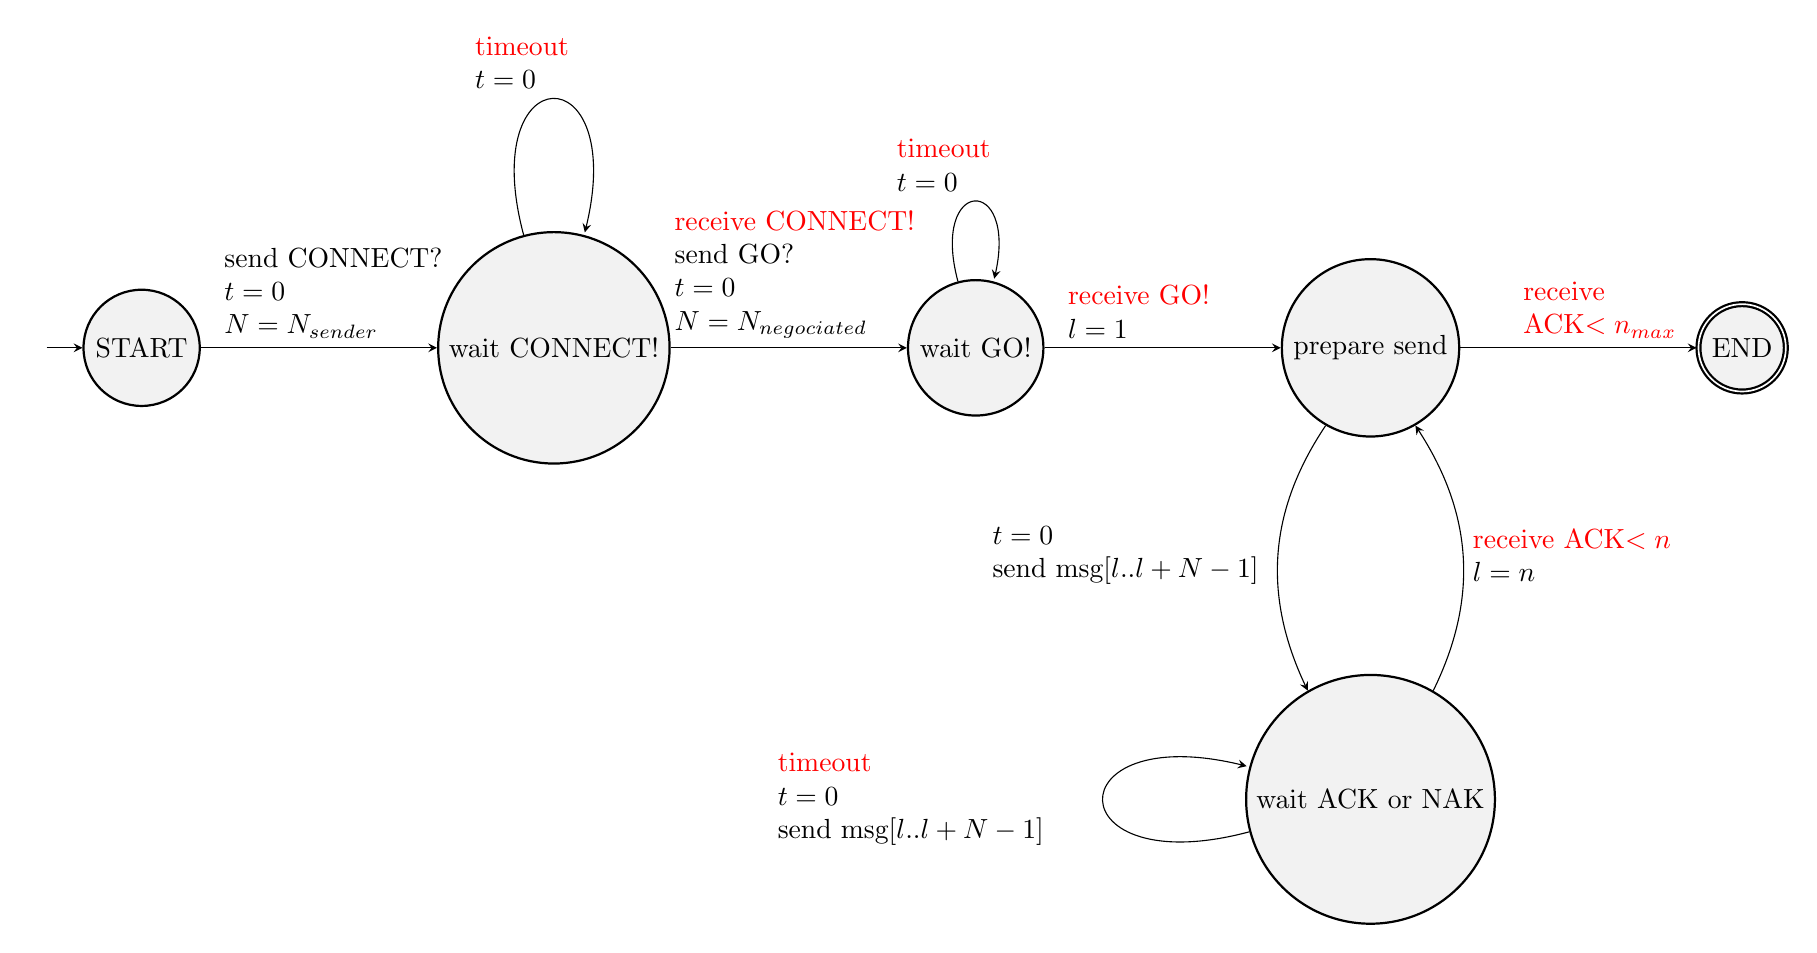
\begin{tikzpicture}
			\node[state, initial] (START) {START};
			\node[state, right=of START] (WAIT0) {wait CONNECT!};
			\node[state, right=of WAIT0] (NEG) {wait GO!};
			\node[state, right=of NEG] (WAIT1) {prepare send};
			\node[state, below=of WAIT1] (WAIT2) {wait ACK or NAK};
			\node[state, accepting, right=of WAIT1] (END) {END};
			
			\draw (START) edge[] node[pos=0.6, above]{\parbox{3cm}{send CONNECT? \\ $t=0$ \\ $N = N_{sender}$ }} (WAIT0);
			\draw (WAIT0) edge[loop above] node[]{\parbox{2cm}{\textcolor{red}{timeout} \\ $t=0$ }} (WAIT0);
			\draw (WAIT0) edge[] node[pos=0.6, above]{\parbox{3.5cm}{\textcolor{red}{receive CONNECT!} \\ send GO? \\ $t=0$ \\ $N = N_{negociated}$ }} (NEG);
			\draw (NEG) edge[loop above] node[]{\parbox{2cm}{\textcolor{red}{timeout} \\ $t=0$ }} (NEG);
			\draw (NEG) edge[] node[pos=0.6, above]{\parbox{3cm}{\textcolor{red}{receive GO!} \\ $l=1$}} (WAIT1);
			\draw (WAIT1) edge[bend right] node[left]{\parbox{3.5cm}{$t=0$ \\ send msg$[l..l+N-1]$}} (WAIT2);
			\draw (WAIT2) edge[loop left] node[left]{\parbox{4cm}{\textcolor{red}{timeout} \\ $t=0$ \\ send msg$[l..l+N-1]$}} (WAIT2);
			\draw (WAIT2) edge[bend right] node[right]{\parbox{3.5cm}{\textcolor{red}{receive ACK$<n$}\\ $l=n$}} (WAIT1);
			\draw (WAIT1) edge[] node[pos=0.6, above]{\parbox{2cm}{\textcolor{red}{receive ACK$<n_{max}$}}} (END);
		\end{tikzpicture}
	\end{figure}
	
	\newpage

	\section{Receiver state machine}
	
	\begin{itemize}
		\item We suppose that the receiver discards all out of order packets. If packet $n$ is lost and receiver sends ACK$<n$ then any out of order packet with sequence number $n$ will be retransmitted, so for the sake of simplicity we can just ignore the previously received out of order packets.
		\item For notation, we use $n$ to denote the sequence number of the next expected packet.
	\end{itemize}
	
	\begin{figure}[ht]
		\centering
		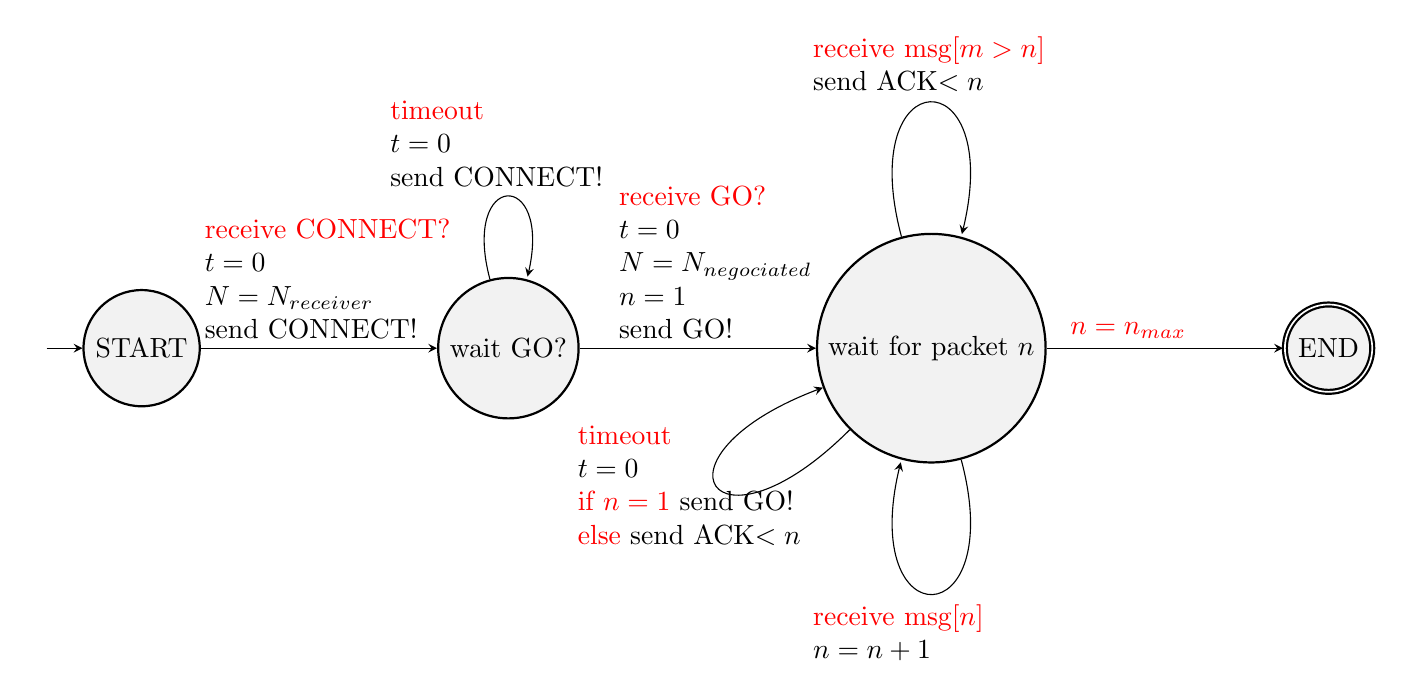
\begin{tikzpicture}
			\node[state, initial] (START) {START};
			\node[state, right=of START] (NEG) {wait GO?};
			\node[state, right=of NEG] (WAIT1) {wait for packet $n$};
			\node[state, accepting, right=of WAIT1] (END) {END};
			
			\draw (START) edge[] node[pos=0.6, above]{\parbox{3.5cm}{\textcolor{red}{receive CONNECT?} \\ $t=0$ \\ $N = N_{receiver}$ \\ send CONNECT!}} (NEG);
			\draw (NEG) edge[] node[pos=0.75, above]{\parbox{3.5cm}{\textcolor{red}{receive GO?} \\ $t=0$ \\ $N = N_{negociated}$ \\ $n=1$ \\ send GO!}} (WAIT1);
			\draw (NEG) edge[loop above] node[]{\parbox{3cm}{\textcolor{red}{timeout} \\ $t=0$ \\ send CONNECT!}} (NEG);
			\draw (WAIT1) edge[loop, out=225, in=200, looseness=10] node[]{\parbox{3.5cm}{\textcolor{red}{timeout} \\ $t=0$ \\ \textcolor{red}{if $n=1$} send GO! \\ \textcolor{red}{else} send ACK$<n$}} (WAIT1);
			\draw (WAIT1) edge[loop below] node[]{\parbox{3cm}{\textcolor{red}{receive msg$[n]$} \\ $n=n+1$}} (WAIT1);
			\draw (WAIT1) edge[loop above] node[]{\parbox{3cm}{\textcolor{red}{receive msg$[m > n]$} \\ send ACK$<n$}} (WAIT1);
			\draw (WAIT1) edge[] node[pos=0.6, above]{\parbox{3cm}{\textcolor{red}{$n = n_{max}$}}} (END);
			
		\end{tikzpicture}
	\end{figure}

\end{document}